\documentclass[preprint]{aastex} 

\usepackage[top=1in, bottom=1in, left=1in, right=1in]{geometry}
\usepackage{amsmath}
\usepackage{graphicx}
\usepackage{mdwlist}
\usepackage{natbib}
\usepackage{natbibspacing}
\usepackage{caption}
\usepackage{subcaption}
\usepackage{enumitem}
\setlength{\bibspacing}{0pt}
\setlength{\parskip}{0pt}
\setlength{\parsep}{0pt}
\setlength{\headsep}{0pt}  
\setlength{\topskip}{0pt}
\setlength{\topmargin}{0pt}
\setlength{\topsep}{0pt}
\setlength{\partopsep}{0pt}
\setlength{\footnotesep}{8pt}
\pagestyle{empty}
\citestyle{aa}
\captionsetup[table]{labelsep=space}
\captionsetup[figure]{labelsep=space}

\newcommand{\simgt}{\stackrel{>}{_{\sim}}}
\def\kperp{k_{\bot}}
\def\kpar{k_{\|}}
\def\k{{\bf k}}
\def\sky{{\theta}}
\def\HI{{H{\small I }}}
\def\HII{{H{\small II }}}
\def\xHI{{x_{\rm\HI}}}

%\usepackage{subfig}
%\usepackage[countmax]{subfloat}

\begin{document}
\title{Project Management Plan}

%A Project Management Plan should be submitted as a supplementary document, and may be up to 
%15 pages in length, although many programs will not need this much space. (Note that the solicitation 
%stated that the management plan should be provided in the Project Description; here we move it to its 
%own supplementary document so that it may be explicitly evaluated by reviewers.)  This section must 
%present a clear and thorough discussion of the project management structure and techniques that will 
%be applied. It may include, for example, a construction plan and schedule, a collaboration management 
%plan, a plan for managing telescope access, or any other pertinent management information. The 
%management plan should identify risks and describe their planned mitigation. If your proposed project 
%would have contributions from sources other than NSF, this section should clearly state both the total 
%cost, and the amount being requested from NSF.  

\section{Collaboration and Governance}
HERA builds upon the organization, tools and collaborations developed within the now
merged PAPER and MWA-US groups, as envisioned in the roadmap developed for New
Worlds, New Horizons decadal survey. In addition to the proposing collaborators in
the {\em List of Partner Institutions}, HERA includes key partners in South Africa
and the UK and is finalizing a collaboration with ASIAA.  Details of the collaboration are 
contained within the Collaboration Agreement and are summarized here.
\begin{table}[h]
\begin{tabular}{| p{.35\textwidth} | p{.6\textwidth} |}\hline
\textbf{Institution (location)} & \textbf{Role} \\ \hline
SKA-SA (Cape Town, SA) & Partner in site development, logistics, support, science. They have been active in supporting PAPER.\\ \hline
University KwaZulu Natal (Durban, SA) & Partner in science and support. They have been active in supporting PAPER.\\ \hline
Cavendish Laboratory (Cambridge, UK) & Partner in development, construction, support and science.  They have been active in supporting PAPER. \\ \hline
Academia Sinica Institute for Astronomy and Astrophysics (Taipei, Taiwan) & Science, development and construction (sub-assemblies and components). \\ \hline
\end{tabular}
\label{tab:otherpartners}
\end{table}

\begin{figure}[h]
\centering
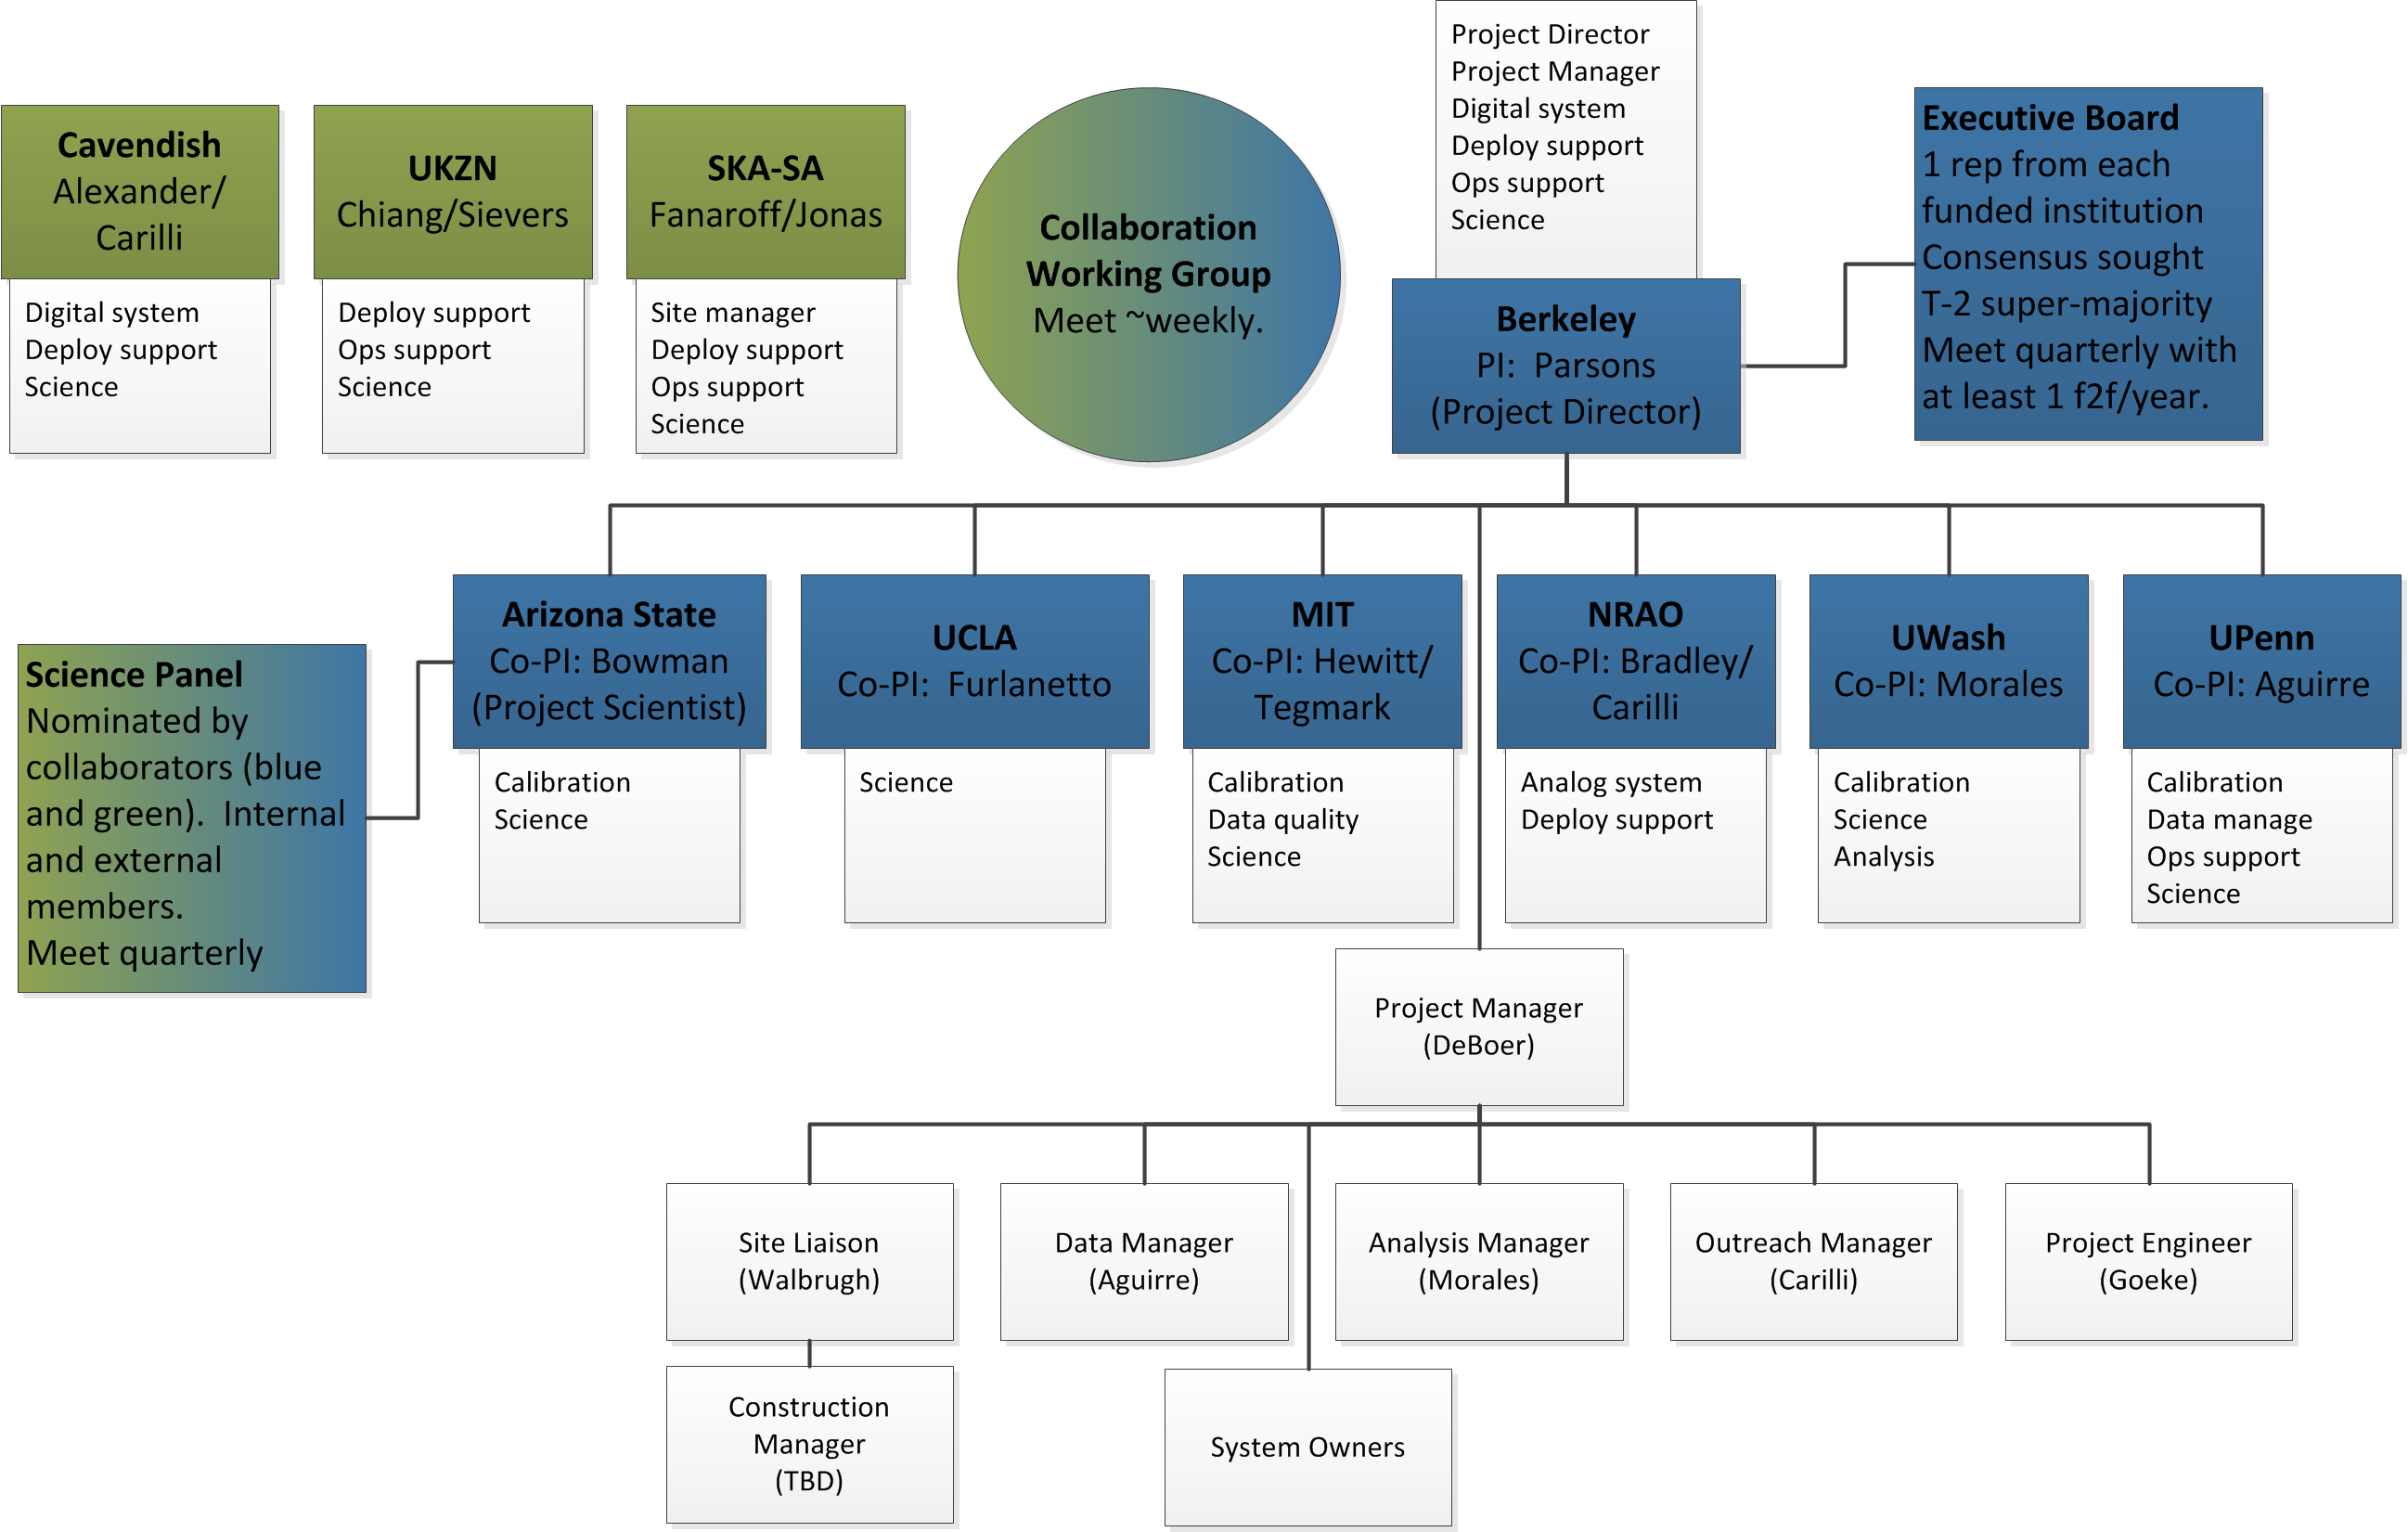
\includegraphics[width=\textwidth]{plots/org.png}
\caption{Org chart showing the collaboration, governance and management.}
\label{fig:org}
\end{figure}

\subsection{Executive Board}
Figure \ref{fig:org} shows the governance and management of the proposed work. The
Executive Board serves as the governing board and has authority over the science
requirements\footnote{{\em Requirements} are the science and operational level
requirements as specified and managed by the Board. {\em Specifications} are the
system requirements specified by the System Owners.}, the scope of the science goals
and milestones. It consists of one voting representative from each of the funded
partners, which typically will be the senior scientific partner at the institution.
The Board is chaired by the Project Director. Though generally operating on
concensus, if matters come to a vote a ``T-2''\footnote{T-2 means that 2 or more must
vote against to defeat a motion.} supermajority will be required. The Executive Board
will meet at least quarterly, with at least one face-to-face meeting per year. The
Board is responsible for producing the NSF annual report. The Board maintains the
list of of Collaborators, which will be maintained on the collaboration website
http://reionization.org.

\subsection{Science Panel}
A Science Panel, chaired by the Project Scientist or designate, will meet at least
quarterly to provide advice on the science (scope, progress, support, ). The
composition is determined by the Executive Board, and membership is open to anybody
the Board deems advisable and is willing to serve. Under the auspices of the Science
Panel, one face-to-face workshop will be held per year, rotating its location among
the partners.

\subsection{Collaboration Working Group}
The Collaboration Working Group comprises individuals named by the partner
institutions and will meet approximately weekly to discuss and review the project. It is chaired
by the Project Director or designate and will discuss any and all relevant aspects of
the project. It represents the primary method of frequent communication between the
partners.


\subsection{Communication}
The core standing meetings for the collaboration have been discussed above, and the
collaboration meeting has been underway for some time. This generally is
conducted by the institutional members being together in a room, and then the groups linked together by a
conferencing system. Berkeley provides full access to the Blue Jeans
network-conferencing system for hosting meetings, including video, simple and
effective desktop sharing, and multiple access methods (computer, phone, networked
video system). Other partners have access to Webex,which is also used. These tools
are routinely used by the partners already and are quite effective.
Other side meetings also occur using these tools, including regular telecons
specifically with South Africa The collaboration makes good use of side-meetings at
professional conferences at which many of the team may be attending.
In addition to meetings, the group obviously makes copious use of e-mail, both direct 
and using a group listserver.  Other tools, such as wikis and web-sites are discussed below.
Good communication is obviously a key ingredient for success.

\section{Management}
The project strives to get the right light level of management over a relatively tight-knit
collaboration.  Most of the construction authority and budget is invested in one location
with oversight by the key senior members of the collaboration.  The analysis and 
scientific tasks are widely spread over the collaboration and are defined at a 
concrete level to assess progress.  General management principles are derived from
{\it A Guide to the Project Management Body of Knowledge} (PMBOK).

Figure \ref{fig:org} shows the management structure.   A Project Manager has
overall responsibility for planning and tracking to achieve the agreed upon
milestones and budget. The Project Manager will brief the Executive Board at each
meeting to summarize the state of the project.  David DeBoer from Berkeley will serve
as the Project Manager.

The Site Liaison is a South African-based person responsible for coordinating activities
between the Collaboration and the broader SKA-SA observatory group.  This link has 
been key in effectively pursuing the PAPER activities in South Africa.  William Walbrugh
will continue to serve as the Site Liaison.  Anita Loots (SKA-SA Deputy Director) serves as a high-level
support contact in South Africa and many other linkages exist between the scientific and managment staffs.

The Data Manager has responsibility for ensuring data quality as archived at the Karoo Array Processor 
Building (KAPB) and the Penn data storage facility.  James Aguirre from Penn will serve as the Data Manager.

The Analysis Manager has responsibility for ensuring that the analysis pipelines are progressing and functioning.
This is further discussed under the Analysis Management section (\ref{sec:analysis}).
Miguel Morales from Washington will serve as the Analysis Manager.

The Project Engineer has responsibilty for ensuring that Components and Systems meet their overall
Specifications and that Interfaces are properly addressed.  Bob Goeke from MIT will serve as the
Project Engineer.

The Outreach Manager will be appointed to track and facilitate the cohort structure of the outreach program.
This person will work closely with a South African counterpart to ensure success of the program.    James
Aguirre from Penn will serve as the Outreach Manager.

\subsection{Project Structure}
The project comprises {\em Components}, which are the physical deliverables, and {\em Systems},
which are logical groupings to achieve a function. Systems may be hardware, software
or both. Systems need not be disjoint collections of Components. Each System has an
{\em Owner}, who is responsible for the System meeting its specifications and satisfying
its interface requirements.

Components will likely span multiple systems. Component owners work with system
owners to meet the components' functional specifications. In practice there is a
great deal of overlap between the components and systems, making this arrangement
practical but it also allows a mechanism to ensure more ``eyes'' on the overall
system as well as regularized reporting. The list of owners resides in the {\tt
ProjectBook} discussed below.

This structure is the organizing principle behind the work breakdown structure and
can be mapped to work package elements and leaders.

\subsection{Project Book and Tools}
The architecture, requirements/specifications, interfaces, budget, milestones, work
breakdown structure, risk register and system documenation are in a common
shared repository, along with processing scripts and collaboration documentation.
This shared repository is referred to as the {\tt ProjectBook}. Architecture,
requirements/ specifications, interface, risk and milestone information reside in a
\LaTeX-based database with full traceability via python and shell scripts for
flow-down throughout the documentation in the {\tt ProjectBook}. Budget and WBS are
in Microsoft Excel and Microsoft Project with python script readers for flow-down
throughout the documentation.

An executive script ensures that all scripts are executed and up-to-date formatted
\LaTeX pdf documentation files are produced. These include auto-generated
architecture, requirement/ specification, interface control, risk register and
milestone documentation, budget and WBS summary documents, as well as flow-down files
into the architecture for traceability. In addition to the auto-generated reports,
System and Component Owners write the narrative documentation referencing the
database items as variables ({\em e.g.} requirements, interfaces, etc). Additional
scripts may be written as needed to access the system for customized reports.

The {\tt ProjectBook} remains the definitive record, but use of a wiki for posting material and hosting
discussions etc is an important component.  The project has full access to wiki tools, and has been
using collaborative wikis in the ongoing collaboration.  The group has a public web-site at http://reionization.org, 
in addition to PAPER and MWA project web-sites at http://eor.berkeley.edu and http://mwatelescope.org respectively.

Additional common repositories host the software developed by the project.  This allows access to all members,
as well as full revision control.  Git/Github is the primary repository tool.  Python is the primary coding/scripting
tool.

Financial tracking is done via the Berkeley Financial System (BFS), supplemented with Excel spreadsheets which are
reconciled by the Project Manager.

Table \ref{tab:softwareTools} lists the primary software tools (management and technical).  Schematics:  visio, technical
\begin{table}[h]
\centering
\caption{Project Software Tools}
\label{tab:softwareTools}
\begin{tabular}{| p{1.3in} | p{4.7in} |}\hline
\textbf{Category} & \textbf{Tools} (primary in bold font) \\ \hline
\raggedright{Documentation} & \textbf{\LaTeX}, Word, {\tt ProjectBook}, pdf \\ \hline
\raggedright{File sharing} & \textbf{Github}, googledocs \\ \hline
\raggedright{Scheduling} & \textbf{MS Project}, {\tt ProjectBook}, ganttProject \\ \hline
\raggedright{Risk register} & {\tt ProjectBook}\\ \hline
\raggedright{Finance} & \textbf{BFS}, Excel, {\tt ProjectBook} \\ \hline
\raggedright{Scripting} & \textbf{Python}, shell \\ \hline
\raggedright{Diagrams} & \textbf{Visio}, Omnigraffle \\ \hline
\raggedright{Mechanical drawings} & \textbf{Autodesk Inventor}, Draftsight \\ \hline
\raggedright{Schematic and layout} &\textbf{Altium Design 6, Mentor Graphics PADS}, Cadence OrCAD \\ \hline
\end{tabular}
\end{table}

\subsection{Change Control}
\label{sec:changecontrol}
Change requests are initiated by an e-mail to the Project Manager indicating the proposed change
and reasons why it is necessary.  Changes may be of the Architecture, Scope, Requirements/ Specifications
Milestones and/or Interface as documented in the Project Book.  The Project Manager will investigate the 
impact of the proposed change and make a recommendation which may be provided to different bodies, 
depending on the scope of the change.  The Project Manager may initiate a change request by appropriately 
formulating and sending on a recommendation.

As mentioned above, the Executive Board controls Requirements, Scope and Milestone change requests
and they receive recommendations regarding these items.  If accepted, the Board will instruct the Project Manager to 
propagate the change within the management system and communicate this change to the partners.

Other change request recommendations will be provided to the impacted Owners of Systems and
Components and accepted on a consensus basis of the impacted Owners and Project Manager.  
In the event that consensus is not reached, the Project Director remains the final arbiter.  The Project 
Director may overrule consensus by approval of the Executive Board.  If accepted, the Project Manager 
will institute the change and communicate appropriately throughout the project.

\section{Array Construction}
\label{sec:construction}
As mentioned above, the construction is approached in phases, with defined functionality (hardware 
and analysis at each stage.  Broadly, these phases are:  (1) preparation and prototyping, (2) HERA-127, 
and (3) HERA-331.  These are summarized in Figure \ref{fig:scheduleSummary}.   HERA-127 uses new
elements, but reusing the PAPER electronics from front-end to correlator.  HERA-331 will build the 
remainder of the elements and incorporate new feeds with expanded frequency coverage, new nodes
(which include the new SNAP boards, which send fiber back to the KAPB), and a new correlator (which
is based completely on the previous deployed correlator).
An overview of the construction is given below.

\subsection{Prototyping}
A number of prototyping activities will take place as part of this work.  A full-size HERA element prototype has been
constructed and is currently under test.  Its primary goals have been to investigate and refine the construction
method and to do some initial reflection tests with various configurations of screening.  The element is shown in
Figure \ref{fig:heraclesANDkaroo}.

A pair of HERA elements will be constructed at the National Radio Astronomy Observatory Green Bank
facility by Green Bank staff under the supervision of PI Rich Bradley.  This prototype will further refine
the design, as well as allow additional reflection and cross-couping tests.  Using them in conjunction 
with PAPER antenna elements will allow initial HERA beam measurements.  These dishes will be used
in the development of the new expanded performance feed elements.

The final element prototypes will be the first three HERA elements at the site and will be the first three of the full
array.  This will be constructed by a joint team of the US staff and the SA staff and possibly by likely vendors.
This will allow final refinement in the South African context with local staff, as well as to train the crew chiefs
and other staff on the process.

The node will be prototyped in Berkeley in advance of the Production Readiness Review to make sure
all bases are covered (shielding, power, thermal, areal, etc).  

\subsection{Karoo}
The primary construction location is in the South African Karoo Astronomy Reserve, where PAPER has been deployed
and operated since 2009 (see Figure \ref{fig:heraclesANDkaroo}).  The South African SKA organization (``SKA-SA'') is a key partner and has a great deal of
infrastructure and support on-site and for the site and a close working relationship exists between the partners.

\begin{figure}[htb]
\centering
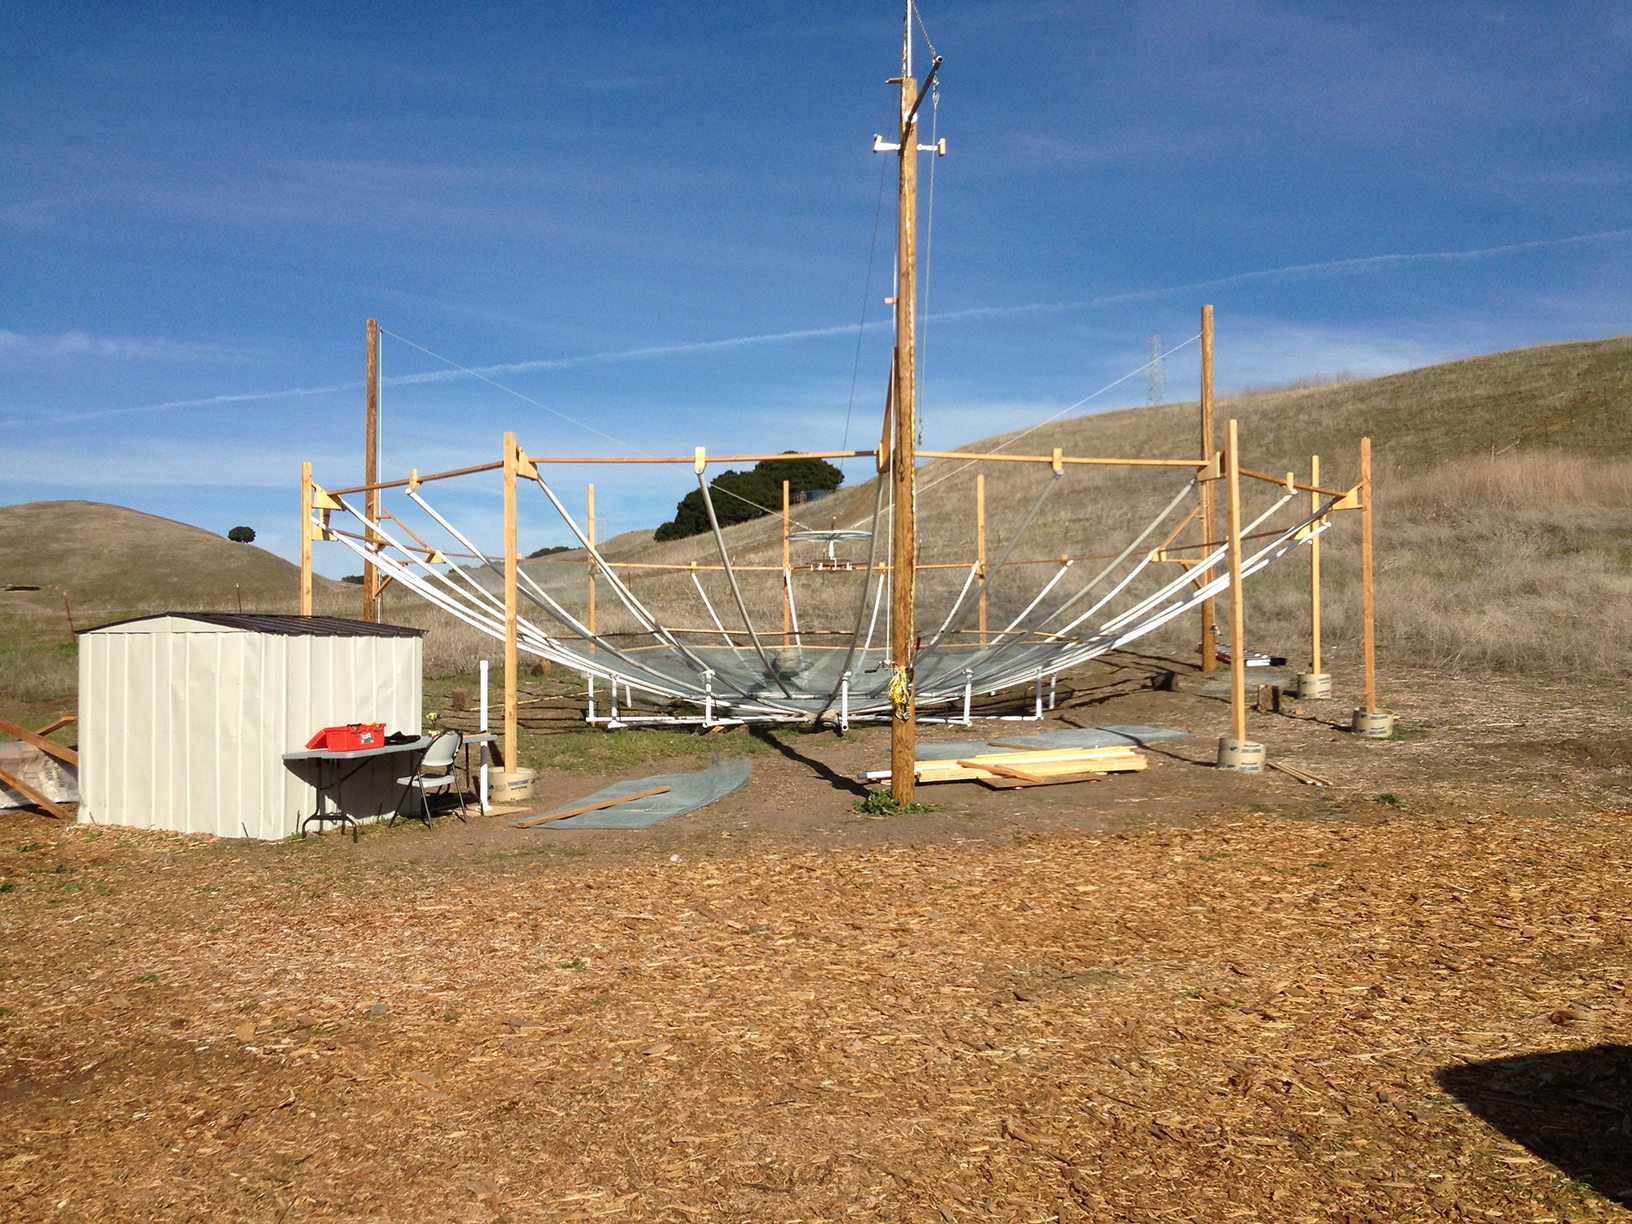
\includegraphics[width=0.45\textwidth]{plots/heracles.png}
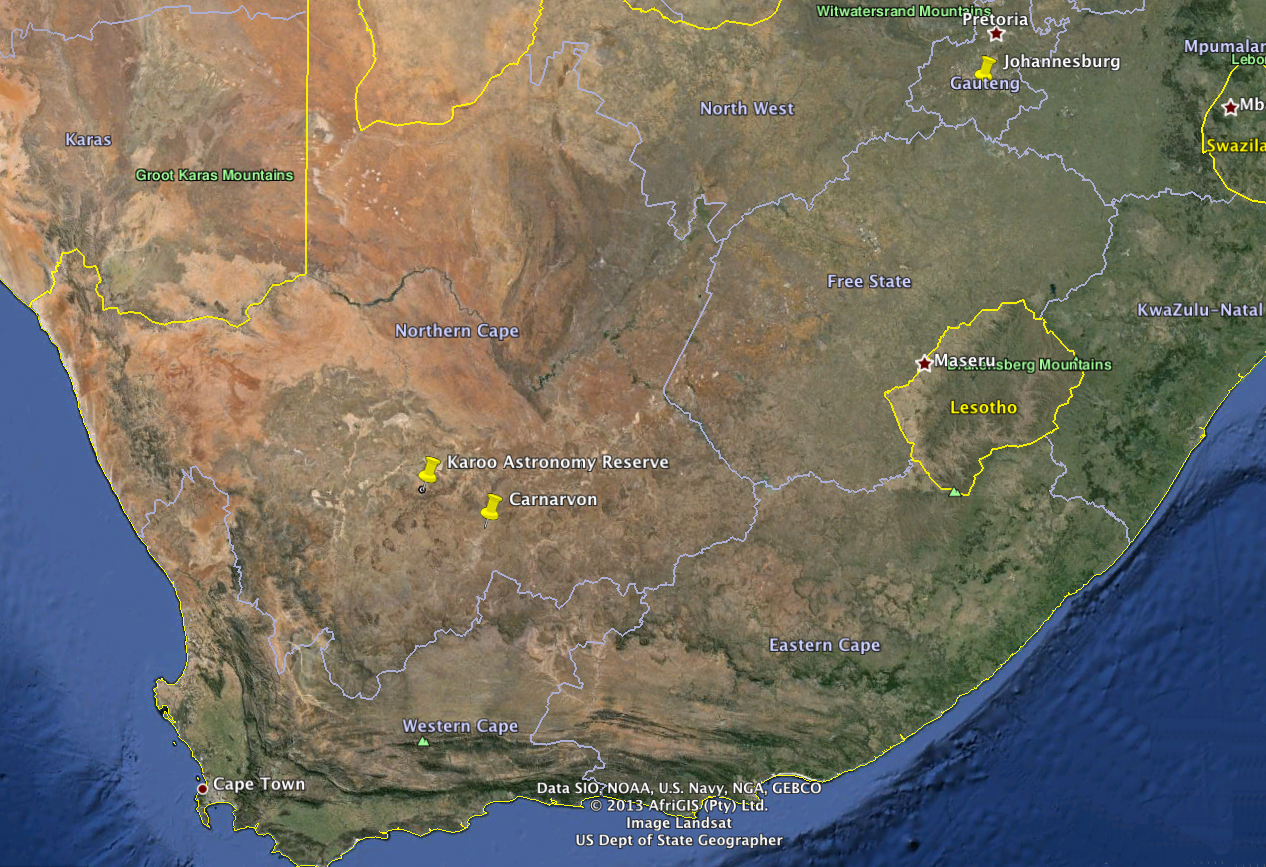
\includegraphics[width=0.51\textwidth]{plots/karoo.png}
\caption{The Berkeley HERA prototype element (left) and the location of the Karoo facility in South Africa.}
\label{fig:heraclesANDkaroo}
\end{figure}

The project is phased in its delivery (see Figure \ref{fig:scheduleSummary}) and
designed such that most sub-assemblies are built off-site and then shipped to site
for subsequent installation. The on-site installation has an overall On-Site Manager
(which rotates among a small number of expert staff) supervising two 6-8 member
crews, each with a crew chief. Primary sub-assemblies are the hub casts, pole/post
end-caps (which hold the surface support spars and rim pieces and contain locational
markers), PVC support sub-assemblies for the surface, feed, feed-backplane, central
cone, and the node enclosure. These are shown in Table \ref{tab:subassycontracts}.

\begin{figure}[htb]
\centering
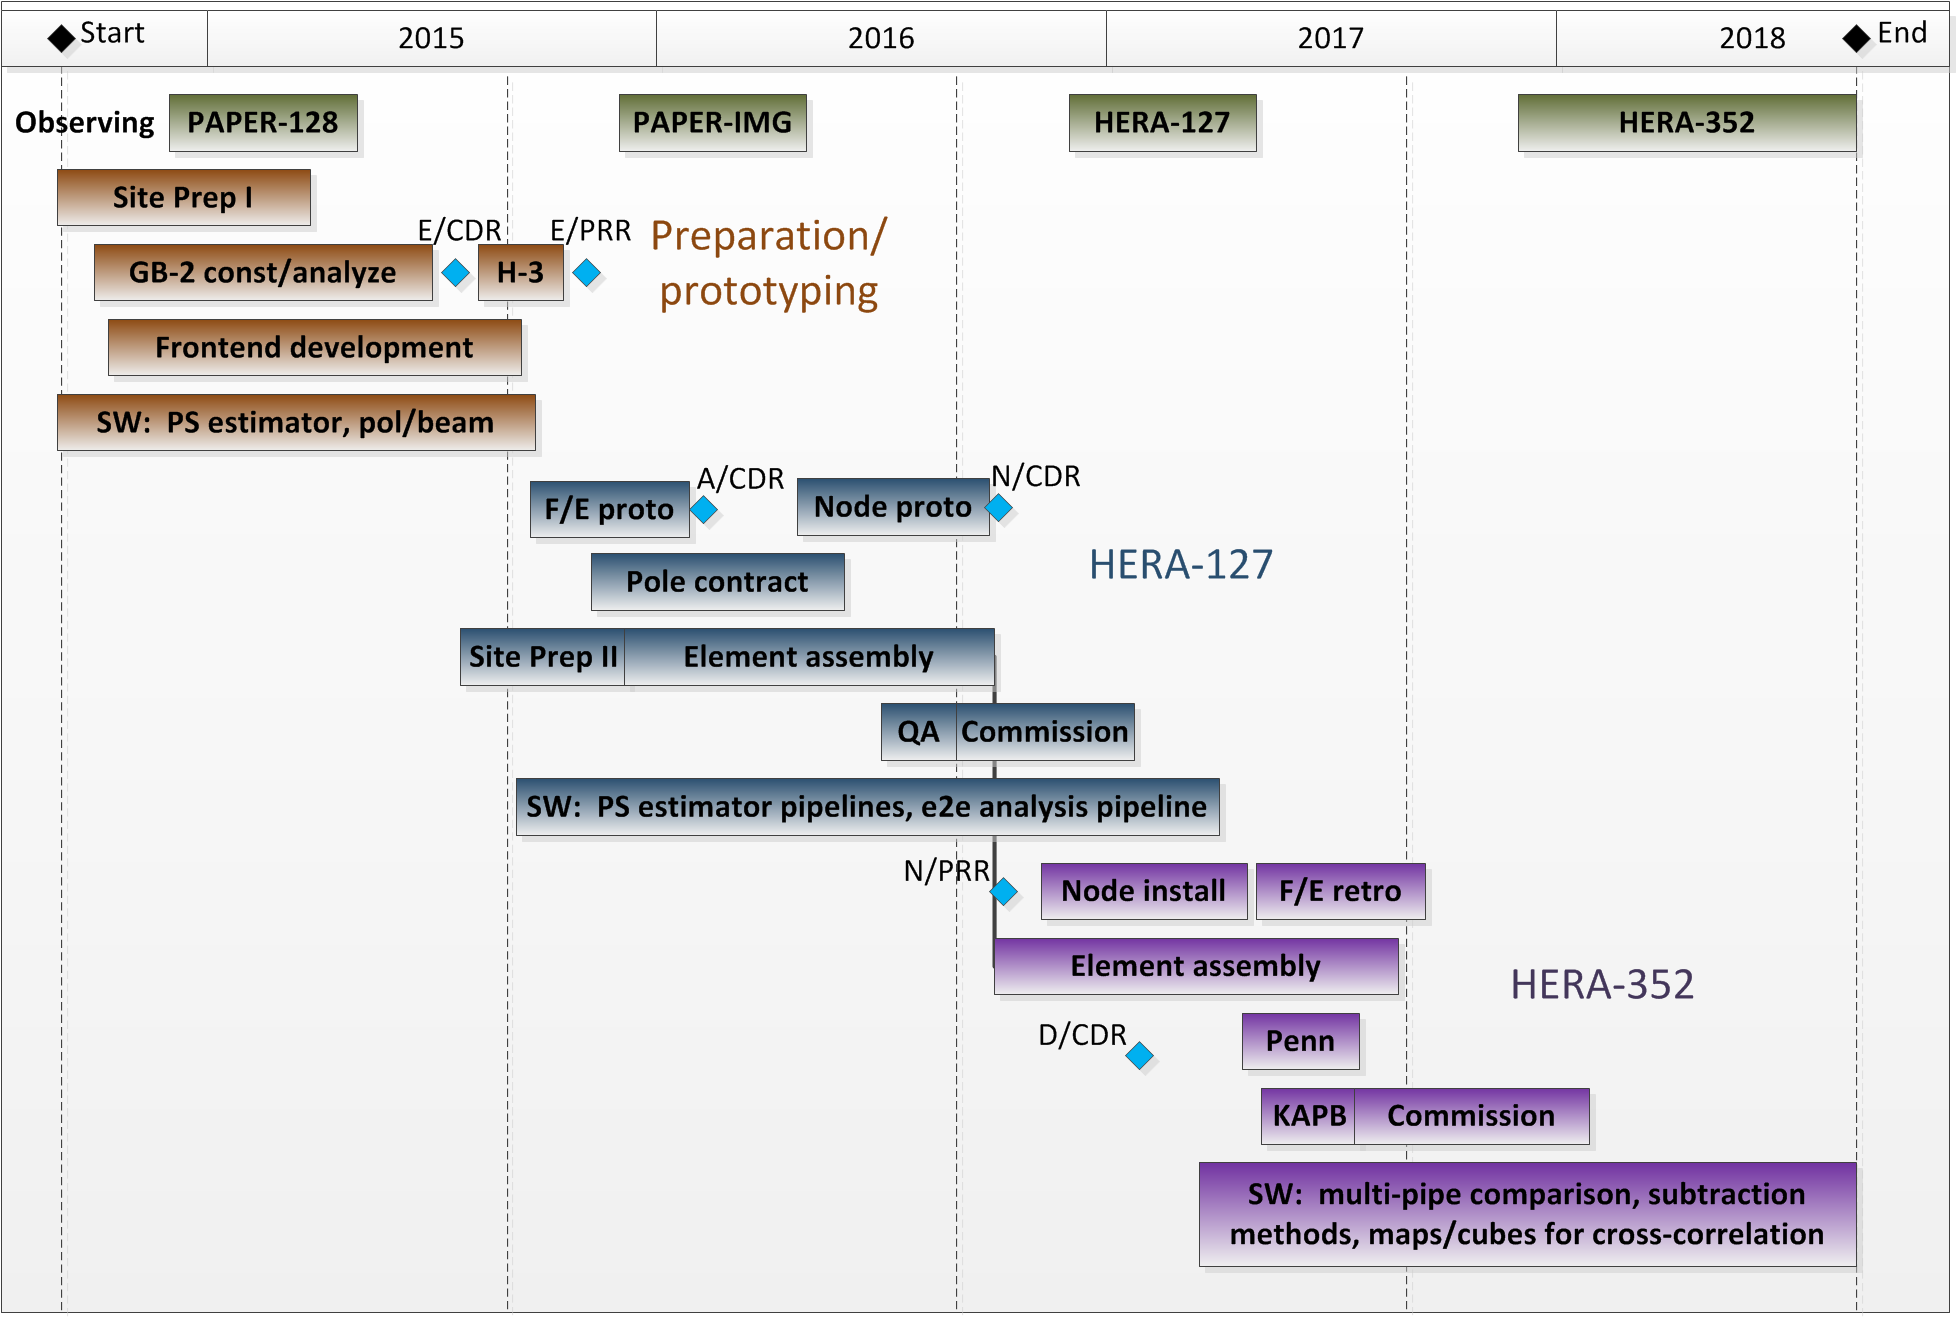
\includegraphics[width=\textwidth]{plots/schedule.png}
\caption{Phases and top-level activities of construction}
\label{fig:scheduleSummary}
\end{figure}

\begin{table}[tbh]
\centering
\caption{Primary sub-assembly contracts} \label{tab:subassycontracts}
\begin{tabular}{| p{1.4in} | p{1.4in} | p{1.4in} | p{1.4in} |}\hline
\textbf{Element} & \textbf{Analog} & \textbf{Digital} & \textbf{Node} \\ \hline
%Element
\raggedright{hub casts, pole/post endcaps, PVC surface support, feed, feed backplane, central cone} &
%Analog
\raggedright{LNA/balun modules, post-amplifier modules, RF cables} &
%Digital
\raggedright{SNAP boards} &
%Node
Enclosure, power handling, air-conditioning. \\ \hline
\end{tabular}
\end{table}

The ordered list of installation is given below. A number in square brackets denotes
a separate contract (or sub-contract), while a single asterisk denotes work that may
be done in parallel by the two teams. An additional team (or teams) may be added to
pace the work, primarily in the build-out from 127 to 331 antenna elements (when there will also be more
experiences members of the team who may step up as crew chiefs). Double asterisks are
activities done with US experts supported by local staff. The first installations
will also involve US-based experts to train the on-site staff, particularly the crew
chiefs.
\begin{enumerate}[itemsep=-3pt]
\item Sub-assembly contracts [1]
\item Grounds preparation and power/fiber reticulation. [2]
\item Pole installation [3,*]
\item Hub installation using centering and hub jigs  [*]
\item Rim/post installation using leveling jig and Total Station [*]
\item Surface support installation [*]
\item Mesh installation [*]
\item Node enclosure [*]
\item Feed installation [*]
\item Node electronics [**]
\item KAPB electronics [**]
\item Penn cluster [**]
\item Commissioning [**]
\end{enumerate}
The overall schedule and milestones are summarized in Section \ref{sec:schedule}.

HERA-127 will use the same electronics as PAPER and commissioning and debugging of the physical
hardware should be straightforward.  Commissioning is more confined to the analysis.  As in PAPER,
the experienced digital team from Berkeley will commission the hardware in the new location.

With HERA-331, the new node electronics begin to be incorporated, so commissioning will involve
other aspects that will utilze both US-based experts, as well as the local experts in Cape Town and Durban.
Commissioning on the nodes will begin with installation of the first node, rather than requiring all nodes
to be installed.

When the new processor is installed and full use of the full signal path is commenced, US-based staff
will spend extensive time on location commissioning the full system.  The system will first be tested in the Berkeley lab.  
Initially, the digital experts will provide full hardware funcationality, then science staff and students will use the system on-site to debug.

\subsection{Penn Cluster}
The other deployed is the computing cluster based at the University of Pennsylvanis, which currently hosts the existing
PAPER cluster {\em Shredder}.  Shredder is adequate for the HERA-127 phase, but a new cluster and storage will be
purchased for HERA-331.  This will be purchased as late as possible to derive maximum benefit from Moore's Law.

\section{Management of Operations}
\label{sec:operations}

Because HERA is a fully-correlated, drift-scan instrument, there are no operational
decisions that need to be made for observing. Hence, HERA does not require a Time
Allocation Committee. Managing routine operation of the HERA instrument consists of
ensuring the functionality of all subsystems and the flow of information between
them. The inclusion of specific Quality Assurance servers (QAservers) greatly
facilitates core functionality. "Observers" will be appointed amongst the
collaborators on a rotating basis, who will manage operations, drawing on the
resources and information available through the monitor and control system. Coverage
will be overseen by the Project Manager. System failures will be identified in real
time and referred to the system owner for diagnosis, repair, and testing.


\section{Analysis Management}
\label{sec:analysis}

One of the absolute key deliverables is an analysis pipeline that can yield the science.  This is the primary area of
research and the greatest scientific risk.  The HERA collaboration has established
a three-tiered ranking system for grouping analysis development activities according to priority and risk.

Tier 1 activities are lower risk, and are considered essential to project success.  Each analysis activity
in this tier is led at a single institution, proceeds according to an established timeline, and is managed
similarly to other essential systems in the project.  Examples of Tier 1 analysis activities include:
establishing a real-time redundancy-based calibration pipeline, interfacing with existing synthesis imaging
software packages to produce images and maps of foregrounds, developing a fully covariant treatment of
the delay-spectrum power spectrum, and applying this pipeline to measuring the power spectrum of reionization
outside of the foreground wedge at high significance.
The Analysis Manager is responsible to evaluating
and managing progress on Tier 1 analysis activities and reporting to the Project Manager.

Tier 2 activities are higher risk, and augment the science case of the project.  Activities in
this tier are spread among institutions, with complementary efforts proceeding in parallel to
reduce risk.  Tier 2 activities proceed according to a more flexible timeline, and are incorporated
into routine analysis pipelines as they become available.  Examples of Tier 2 analysis activities
include:
developing alternate imaging pipelines aimed at suppressing systematics within the foreground wedge
to gain higher significance power spectrum detections over a broader range of scales, developing
techniques to directly image reionization structures, and exploring whether HERA measurements at
higher redshifts can be used to produce meaningful constraints on the state of the IGM during
our cosmic dawn prior to reionization.  The Analysis Manager is responsible for managing and coordinating
parallel Tier 2 analysis activities, and reporting progress to the Project Manager.

Finally, Tier 3 includes analysis activities that are considered ancillary or too risky to
be included in HERA's focused science case.
Activities in these areas are not supported directly under this proposal, but may be pursued as
contributed efforts by associated institutions.  Examples of Tier 3 analysis activities include
ionospheric studies, surveying for transient events, other miscellaneous foreground studies, and
examination of higher-order statistics of reionization.  While not directly supported by this proposal,
these activities will nonetheless report progress to the Analysis manager to ensure
robust communication of active analysis efforts within the HERA collaboration.

Inheriting from the MWA, HERA will hold annual ``busy weeks'', organized by the Analysis Manager in
conjuction with the annual project meetings.  These busy weeks gather a critical
mass of collaborators engaged in the development of analysis software together in a manner conducive to
transferring expertise and sharing software and science interactively.  Busy weeks will typically
have a priority list of development activities, set by the Analysis Manager, that will be 
focused on, with many collaborators contributing
ideas and code toward these priority activities.

\section{Reviews}
\label{sec:reviews}
In order to assess project progress and ensure that adequate scope and function is achieved,
the project will have a series of reviews on key components.

Preliminary Design Reviews (PDR) for the major systems will be held as special meetings 
of the Collaboration Working Group.  Each system owner will be responsible for organizing
a PDR at least two months in advance of the appropriate CDR.  Notes from the PDR will be
kept and distributed among the collaborators.

Critical Design Reviews (CDR) organized by the Project Manager/Engineer will be 
held for the major items:  
\begin{itemize}[noitemsep,nolistsep]
\item element - Y1, Qtr 4
\item analog - Y2, Qtr 2
\item node - Y3, Qtr 1
\item digital/datahandling Y3, Qtr 2
\end{itemize}

The CDR panel will be composed of 1-3 external reviewers, along with the Project
Director, Project Scientist and a representative
from the Executive Board. It will be chaired by an external reviewer. The panel
report and its response will be open documents.

A Production Readiness Review will be held before issuing major contracts.  These will
be organized by the Project Manager and include at least one external expert.  Currently, these
only relate to the Element and Node.


\section{Budget Summary}
\label{sec:budget}
A thorough ``bottoms-up'' costing exercise has been underway for sometime. The
equipment costing is informed by (1) the construction of a full-size prototype, which
is currently being completed and is under test as features are added; (b) costing
done by the South African developers based on actuals at the Karoo site; (c)
extensive design and cost experience of CASPER hardware; and (d) the previous PAPER
and MWA deployments, which have very similar analog and digital components. Included
in the equipment cost is labor to produce sub-assemblies and install on-site. The
equipment budget is summarized in Table \ref{tab:budgetsummary} and totals
\$5,672,384

\begin{table}[t]
\centering
\caption{System Cost Summary}
\label{tab:budgetsummary}
\begin{tabular}{| p{2in} | p{2in} | p{2in} | } \hline
\noindent
\textbf{Element:}  \$2,064,411
\vspace{-0.1in}
\begin{itemize}[parsep=-2pt, itemsep=-3pt]
\item Misc:   \$170,474
\item Hub:   \$26,400
\item Support:   \$576,426
\item Surface:   \$729,696
\item Labor:   \$481,416
\item Shipping:   \$80,000
\vspace{-.1in}
\end{itemize}
 &
 \noindent
\textbf{Frontend:}  \$498,487
\vspace{-0.1in}
\begin{itemize}[parsep=-2pt, itemsep=-3pt]
\item Misc:   \$5,000
\item Feed:   \$120,384
\item LNA:   \$293,959
\item RFcable:   \$64,064
\item Power:   \$7,040
\item Labor:   \$7,040
\item Shipping:   \$1,000
\vspace{-.1in}
\end{itemize}
 &
 \noindent
\textbf{Node:}  \$1,254,981
\vspace{-0.1in}
\begin{itemize}[parsep=-2pt, itemsep=-3pt]
\item Misc:   \$26,000
\item Enclosure:   \$123,500
\item Receiver:   \$601,061
\item DAQ:   \$206,144
\item Control:   \$52,000
\item Fiber:   \$78,000
\item Power:   \$45,500
\item RFcable:   \$83,776
\item Labor:   \$13,000
\item Shipping:   \$26,000
\vspace{-.1in}
\end{itemize}
\\ \hline
\noindent
\textbf{Container:}  \$834,425
\vspace{-0.1in}
\begin{itemize}[parsep=-2pt, itemsep=-3pt]
\item Misc:   \$5,000
\item Fibre:   \$129,787
\item Power:   \$425,300
\item Timing:   \$15,000
\item Site:   \$228,838
\item Control:   \$500
\item Shipping:   \$30,000
\vspace{-.1in}
\end{itemize}
 &
 \noindent
\textbf{KAPB:}  \$579,079
\vspace{-0.1in}
\begin{itemize}[parsep=-2pt, itemsep=-3pt]
\item Misc:   \$5,000
\item Datahandling:   \$239,954
\item Processor:   \$228,200
\item Control:   \$3,000
\item Fiber:   \$47,200
\item Power:   \$30,225
\item Labor:   \$15,500
\item Shipping:   \$10,000
\vspace{-.1in}
\end{itemize}
 &
 \noindent
\textbf{Computing:}  \$441,000
\vspace{-0.1in}
\begin{itemize}[parsep=-2pt, itemsep=-3pt]
\item Misc:   \$24,000
\item Cluster:   \$115,000
\item Storage:   \$300,000
\item Server:   \$2,000
\vspace{-.1in}
\end{itemize}
\\ \hline
\end{tabular}
\end{table}


The staffing exercise has also been underway for sometime and is informed by a robust
``bottoms-up'' work breakdown by task and by institution. A summary is given in Section \ref{sec:wbs}.
The overall budget is given in Table \ref{tab:expenses}.  This represents the full cost of the project


\begin{table}[h]
\centering
\caption{Expenses summary}
\label{tab:expenses}
\begin{tabular}{| p{0.5in} | p{.6in} |  p{.6in} |  p{.6in} |  p{.6in} |  p{.6in} |  p{.6in} |  p{.6in} |  p{.6in} | }\hline
  k\$   & \textbf{Berkel} & \textbf{Penn} & \textbf{MIT} & \textbf{UW} & \textbf{ASU} & \textbf{UCLA} & \textbf{NRAO} & \textbf{TOTAL}\\\hline
\textbf{Salary}&       2,834  &         420  &         760  &         365  &         557  &         213  &         201  &       5,350  \\\hline
\textbf{Equipm}&       5,231  &         441  &          35  &          10  &          21  &           0  &          77  &       5,815  \\\hline
\textbf{Other}&         768  &         274  &         181  &         126  &         163  &          65  &          10  &       1,588  \\\hline
\textbf{Indire}&       2,027  &         307  &         437  &         129  &         353  &         116  &          20  &       3,388  \\\hline
\textbf{TOTAL}&      10,861  &       1,442  &       1,413  &         630  &       1,094  &         393  &         308  &      16,141  \\\hline
\end{tabular}
\end{table}


\section{Schedule Summary}
\label{sec:schedule}
The schedule is primarily tracked by setting a fairly large number of high-level
milestones that get tracked in the {\tt ProjectBook}. These map to staff in a work
breakdown schedule, which is tracked in MS Project. The high-level milestones are
listed below, which amplifies on Figure \ref{fig:scheduleSummary}.


%%%%%%%%%%%%%%%%%%%%%%%%%%%%%FOCUS ON BELOW%%%%%%%%%%%%%%%%%%%%%%%%%%%%%%%
\begin{itemize}[itemsep=-4pt,parsep=-3pt]
\item Year 1:  Infrastructure, Prototyping, Contract Preparation (FY 2015).
\begin{itemize}[itemsep=-4pt]
\item Install basic infrastructure (ground leveling, power, network connectivity) for new infrastructure
\item Incorporate existing PAPER-128 antennas, correlator, and housing container. 
\item Install additional prototypes in Green Bank and test.
\item Define final design package for element construction
\item Start developing improved HERA baluns, receivers, feeds, nodes, and in-situ antenna calibration system. 
\item Continue delay-spectrum, FHD, and optimal estimator software development.
\item Develop polarization capable software for beam/leakage studies.
\end{itemize}
\item Year 2:  Hardware Commissioning and Deep Foreground Survey (FY 2016). 
\begin{itemize}[itemsep=-4pt]
\item Observations using PAPER antennas in an imaging configuration. 
\item Determine on-sky beam response of HERA antennas to facilitate future source subtraction efforts. 
\item Finalize site infrastructure (high-bandwidth optical network, surveying, trenching). 
\item Commission new feeds, receivers, nodes, and calibration systems in Green Bank and SA. 
\item Complete HERA-127 construction
\item Initial delay-spectrum, FHD, and optimal estimator software ready for HERA 127 analysis.
\item Full end-to-end simulations of analysis pipelines.
\end{itemize}
\item Year 3:  HERA 127 and Detecting the Rise and Fall of Reionization (FY 2017). 
\begin{itemize}[itemsep=-4pt]
\item HERA 127 complete. Science observations begin using the PAPER correlator. 
\item Begin deployment of HERA 331. Install new node electronics and a 331-element, GPU-based correlator in the Karoo Array Processing Building (KAPB). 
\item Install new data storage infrastructure in the KAPB. 
\item Upgrade the UPenn analysis cluster. 
\item Finish construction of HERA 331
\item Apply proven delay-spectrum analysis techniques to HERA 127 observations to constrain the timing and duration of reionization. 
\item Multi-pipeline analysis of HERA 127 observations to compare pipeline strengths/weaknesses.
\end{itemize}
\item Year 4:  HERA 331 and Measuring the Evolution of the First Galaxies (FY 2018). 
\begin{itemize}[itemsep=-4pt]
\item HERA 331 complete. Begin science observations Oct. 2017. 
\item Begin multi-pipeline analysis of data to characterize the evolution of the power spectrum and determining properties of the first galaxies. 
\item Continue analysis software development: optimize existing algorithms and develop imaging-based subtraction techniques for expanding the EoR window
\item Create high-fidelity maps/data cubes of the HERA field for cross-correlation studies
\item Cosmological simulations for extracting reionization physics from power spectrum measurements
\end{itemize}
\end{itemize}

\section{WBS Summary}
\label{sec:wbs}
The labor estimate was generated from a very detailed ``bottom's up'' task summary, which maps to the milestones to generate the work breakdown structure.

\section{Risk}
\label{sec:risk}
Risk manifests itself in two broad categories: (1) construction/array risks and (2)
analysis/science risks. The risks to actually achieving the overall outcomes are
primarily contained within the analysis/science risks. Construction/array risks are
more manifest, but are generally addressable by changes in budget (some
reprioritization or de-scoping) or schedule (re-phasing, possibly leveraging more of
the PAPER signal path early etc).

As mentioned above, risk is recorded and tracked in the {\tt ProjectBook} which has tools 
to list and flowdown risk records into the documentation.  The risk register will be 
maintained and updated if necessary and regular reports will be generated by the
{\tt ProjectBook} scripting system.

The white paper that the HERA collaboration generated for the NWNH decadal survey identified nine
primary risks:  RFI, antenna performance, large-N correlation, real-time calibration and imaging, 
ionospheric distortion, Faraday rotation, foreground subtraction and instrument deconvolution.
Of these, most are now well-understood and/or greatly reduced.  The key one in this regard is
the understand of the ``wedge'' and the now demonstrated foreground avoidance techniques.
Retirement of this risk is one key motivator for proceeding with this proposal in this
timeframe.  Large-N correlation and real-time calibration and imaging is also largely a
retired risk, as evidenced by many arrays now deployed around the world.  Ionospheric
distortion issues have not been an issue for existing arrays, a result which will hold for
HERA given the design heritage.  The principle remaining risk relates to polarization leakage.

The following sections will briefly discuss project risks.  The risk register will continue to be
actively maintained in the {\tt ProjectBook}.

\subsection{Analysis/Science Risk}
As in addressing risk on the hardware development, the analysis will proceed in
phased stages as described Section \ref{sec:analysis}. The now well-understood
delay-space approach will be implemented from the start, and the sensitivity of HERA
is such that this approach should yield much of the science. If the foreground
subtraction techniques can be made to work, then the science is greatly enhanced.

As mentioned above in the context of the white paper, polarization leakage is a key
risk to all of the approaches.  To help reduce this risk, this is a key early focus on understanding and
constraining the impacts of the instrumental response via the prototypes.

Increased RFI as the SKA-SA construction activities continue to be on-going and 
ramp up is a risk.  HERA will only observe at night, so active construction will be
minimal during observing periods, and RFI will be more confined to workers quarters.
The location of HERA is therefore closer to future arrays (which have stringent
RFI requirements) and further from any construction camps.  The area resides in
a robust spectrum management zone, and the SKA-SA is very committed to
keeping the site RFI characteristics excellent.  They have a full-time RFI monitor
who is fully supported by on-site staff and they are very proactive in monitoring
and investigating issues.

\subsection{Construction/Array Risk}
The primary risks associated with the construction and operation of the array relate
to the remote location, both in construction and operation. This is largely mitigated
by the amount of infrastructure and support provided by SKA-SA in their activities.

The technology and construction itself is all low risk, as it is either fairly standard and/or
has been used by team members at location.  A new board under development (the Smart Networked
ADC Processor, SNAP, is currently in layout) has some risk since it is not complete, however there
is a robust fall-back to use the existing set of CASPER boards that are currently in use on-site for this
purpose.  As mentioned above, the primary risk here is in cost of building in a remote location.
There are two primary mitigations to this risk:  accruing additional partners who can help bear
the cost risk and descoping the array.

Delays in deplying the SNAP board and node are
mitigated by initially using the existing PAPER-128 system, which can accommodate the first 
HERA-127 phase.  Delays in deploying up-to a target (e.g. 127, 331, 352) can be handled by
observing with the existing antennas while the reminder are deployed.  This means that the
construction approach will be to produce smaller tranches of working elements on a node-by-node
basis, rather than relying on completing every element on a full assembly line basis.

To keep the construction cost low the philosophy has been to maintain/repair rather
than attempt to make it bullet-proof. This means that severe weather could damage the
elements. Experience with the PAPER dipoles has been excellent in this regard, and no
severe wind or water damage has been noticed. Given the readily accessible
construction materials, damage is relatively cheap to fix. For minor damage, local
staff can likely repair (and in a large array, we can handle some non-functional
elements), while major damage would likely need a trip and assessment by US-based
experts.

\end{document}
